% CVPR 2022 Paper Template
% based on the CVPR template provided by Ming-Ming Cheng (https://github.com/MCG-NKU/CVPR_Template)
% modified and extended by Stefan Roth (stefan.roth@NOSPAMtu-darmstadt.de)

\documentclass[10pt,twocolumn,letterpaper]{article}

%%%%%%%%% PAPER TYPE  - PLEASE UPDATE FOR FINAL VERSION
% \usepackage[review]{cvpr}      % To produce the REVIEW version
\usepackage{cvpr}              % To produce the CAMERA-READY version
%\usepackage[pagenumbers]{cvpr} % To force page numbers, e.g. for an arXiv version

% Include other packages here, before hyperref.
\usepackage{graphicx}
\usepackage{amsmath}
\usepackage{amssymb}
\usepackage{booktabs}
\usepackage{CJKutf8}


% It is strongly recommended to use hyperref, especially for the review version.
% hyperref with option pagebackref eases the reviewers' job.
% Please disable hyperref *only* if you encounter grave issues, e.g. with the
% file validation for the camera-ready version.
%
% If you comment hyperref and then uncomment it, you should delete
% ReviewTempalte.aux before re-running LaTeX.
% (Or just hit 'q' on the first LaTeX run, let it finish, and you
%  should be clear).
\usepackage[pagebackref,breaklinks,colorlinks]{hyperref}

\usepackage{pifont}
\usepackage{xcolor}
\newcommand{\cmark}{\textcolor{green!80!black}{\ding{51}}}
\newcommand{\xmark}{\textcolor{red}{\ding{55}}}

% Support for easy cross-referencing
\usepackage[capitalize]{cleveref}
\crefname{section}{Sec.}{Secs.}
\Crefname{section}{Section}{Sections}
\Crefname{table}{Table}{Tables}
\crefname{table}{Tab.}{Tabs.}


%%%%%%%%% PAPER ID  - PLEASE UPDATE
\def\cvprPaperID{*****} % *** Enter the CVPR Paper ID here
\def\confName{CVPR}
\def\confYear{2022}


\begin{document}

%%%%%%%%% TITLE - PLEASE UPDATE
\title{QuickDraw Doodle Classification}

\author{
MaoSiang Chen, ChengHsun Wang, Author3\\
NYCU CS\\
{\tt\small \{siang, simon0525\}.cs09@nycu.edu.tw}
% For a paper whose authors are all at the same institution,
% omit the following lines up until the closing ``}''.
% Additional authors and addresses can be added with ``\and'',
% just like the second author.
% To save space, use either the email address or home page, not both
%
}


\maketitle

%%%%%%%%% ABSTRACT
\begin{abstract}
%   The ABSTRACT is to be in fully justified italicized text, at the top of the left-hand column, below the author and affiliation information.
%   Use the word ``Abstract'' as the title, in 12-point Times, boldface type, centered relative to the column, initially capitalized.
%   The abstract is to be in 10-point, single-spaced type.
%   Leave two blank lines after the Abstract, then begin the main text.
%   Look at previous CVPR abstracts to get a feel for style and length.
The AI game ``Quick, Draw!'' was developed and released by Google in 2016, 
which was made as an experimental game. 
The game asks players to draw a doodle in certain categories,
and it will predict the result by the model behind. 
In this final project, 
we want to find the best way to train models for the doodle classification problem. 
We have trained models with different neural networks, hyperparameters, 
and the size of training dataset to predict the doodles correctly. 
Precisely, we compare the results between different batch size and size of training dataset.
To train the network faster, 
a lighter model MobileNet is used and the input images are in Grayscale.
To reduce RAM usage, we decided to use simplified data and generator for generating training data.
Last but not least, we compared the results and found out a better way to train the model.

\end{abstract}

%%%%%%%%% BODY TEXT



\section{Introduction}
% When writing your introduction, please think about the following questions:

% \begin{itemize}
%     \item What is the problem the paper is trying to tackle?
% \item Why this is an important problem?
% \item Why the problem is challenging?
% \item What are the existing approaches?
% \item What are the limitations of the existing approaches?
% \item What is the proposal of this paper?
% \item How you prove your proposal is effective?
% \end{itemize}

% These questions are essential for readers to understand the motivation of the authors. Please think deeply before writing your final report.

Nowadays, many computer classification-based applications arise, such as handwriting recognition and speech recognition.
There are lots of algorithms used to classify images, CNN is the one that is used most for its great performances.
To train CNN to classify images well, it's important to set the batch size appropriately.
Batch size will affect the performance of CNN and its time to converge, so it is necessary to set according to different situations and the needs.~\cite{BATCHSIZE}
Definitely, training data also influences the training process.
Sometimes, dataset is too large to train each image on our model due to our limited computing resources.
This makes us need to choose parts of the dataset as our training data.
In this study, we want to compare how batch size and the size of training data influence the performance of our model on doodle classification.
In the experiment, we use MobileNet~\cite{MobileNet} as our structure for its lighter structure and efficiency.
For the dataset, we use the QuickDraw dataset on the kaggle, which is a doodle classification dataset.


% Doodle classification is an interesting but not always easy problem because not everyone is good at doodling.
% Take Gartic for example, it's a popular game about guessing what other players draw.
% We can find that it's a little challenging sometimes.
\section{Related Work}
We refer to two papers~\cite{BATCHSIZE,Medical} about CNN performances on different learning rate and batch size. 
One is real world photo classification, and the other is medical picture classification.
These two papers help us realize how to set hyperparameters and have some ideas about batch size.\\

MobileNet is proposed by Google. 
It's based on a streamlined architecture that uses depthwise separable convolutions to build light weight deep neural networks.
The details about it can refer to the paper~\cite{MobileNet}.
When we were choosing on which model to use, we test for both ResNet and MobileNet.
However, MobileNet performs much better than ResNet with the same training conditions.
Therefore, we choose MobileNet as our network.


\section{Methodology}
The training process of CNN can be defined as minimizing a loss function. In our project,
we use cross-entropy loss, which is used as loss function for classification problems most of the time.
The cross-entropy represents the sum of the uncertainty of each category, 
which can be considered as the performance of a model better than error-based loss functions. \\

For training data, we pick certain number of rows from each category and shuffle them into several files. 
Make sure that every batch of training data is fully shuffled. 
To reduce RAM usage, we use generator to provide a batch size of training data. 
Because the input data are raw strokes, 
we turn the strokes into numpy arrays of images by opencv functions. For the prediction result,
we create an one hot encoder to turn a category into a corresponding vector with size (340,1). \\

Then, we generate a validation set with size 1:10 to the size of training data in each epoch.
Since the size of training data in each epoch is 500*680=340000, 
the size of the validation set will be 34000. 
In training phase, we set two callbacks functions, they are \verb|ReduceLROnPlateau| and \verb|ModelCheckpoint|.
The first function will reduce the learning rate by multipling 0.75 if the top 3 accuracy 
of the validation set doesn't increase in three epochs. For the second function,
it will save the best model during the training phase based on the top 3 accuracy on validation set. \\

In order to determine the performance of a model, we generate predictions and submit to Kaggle for scoring.
First, we load weights of the best model in the training phase and predict with strokes in test\_simplified.csv.
Second, we turn the one hot vector into category ID and then the corresponding category.
Finally, save the csv file and submit to Kaggle for scoring.


\section{Experiments}
\begin{itemize}
\item Batch size \\
We have tried two kinds of batch size, which are 340 and 680 each batch. 
As you can see, the loss of validation set with smaller training batch size flucturates more in the training phase. 
However, the one with smaller batch size get higher scores in Kaggle submission. 
\graphicspath{{./images}}
\begin{figure}[!htb]
    \centering
    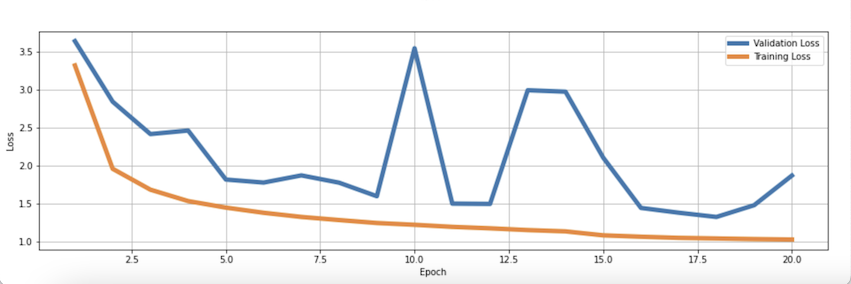
\includegraphics[width=0.8\linewidth]{340-loss.png}
    \caption{The Loss with batch size 340}
\end{figure}
\begin{figure}[!htb]
    \centering
    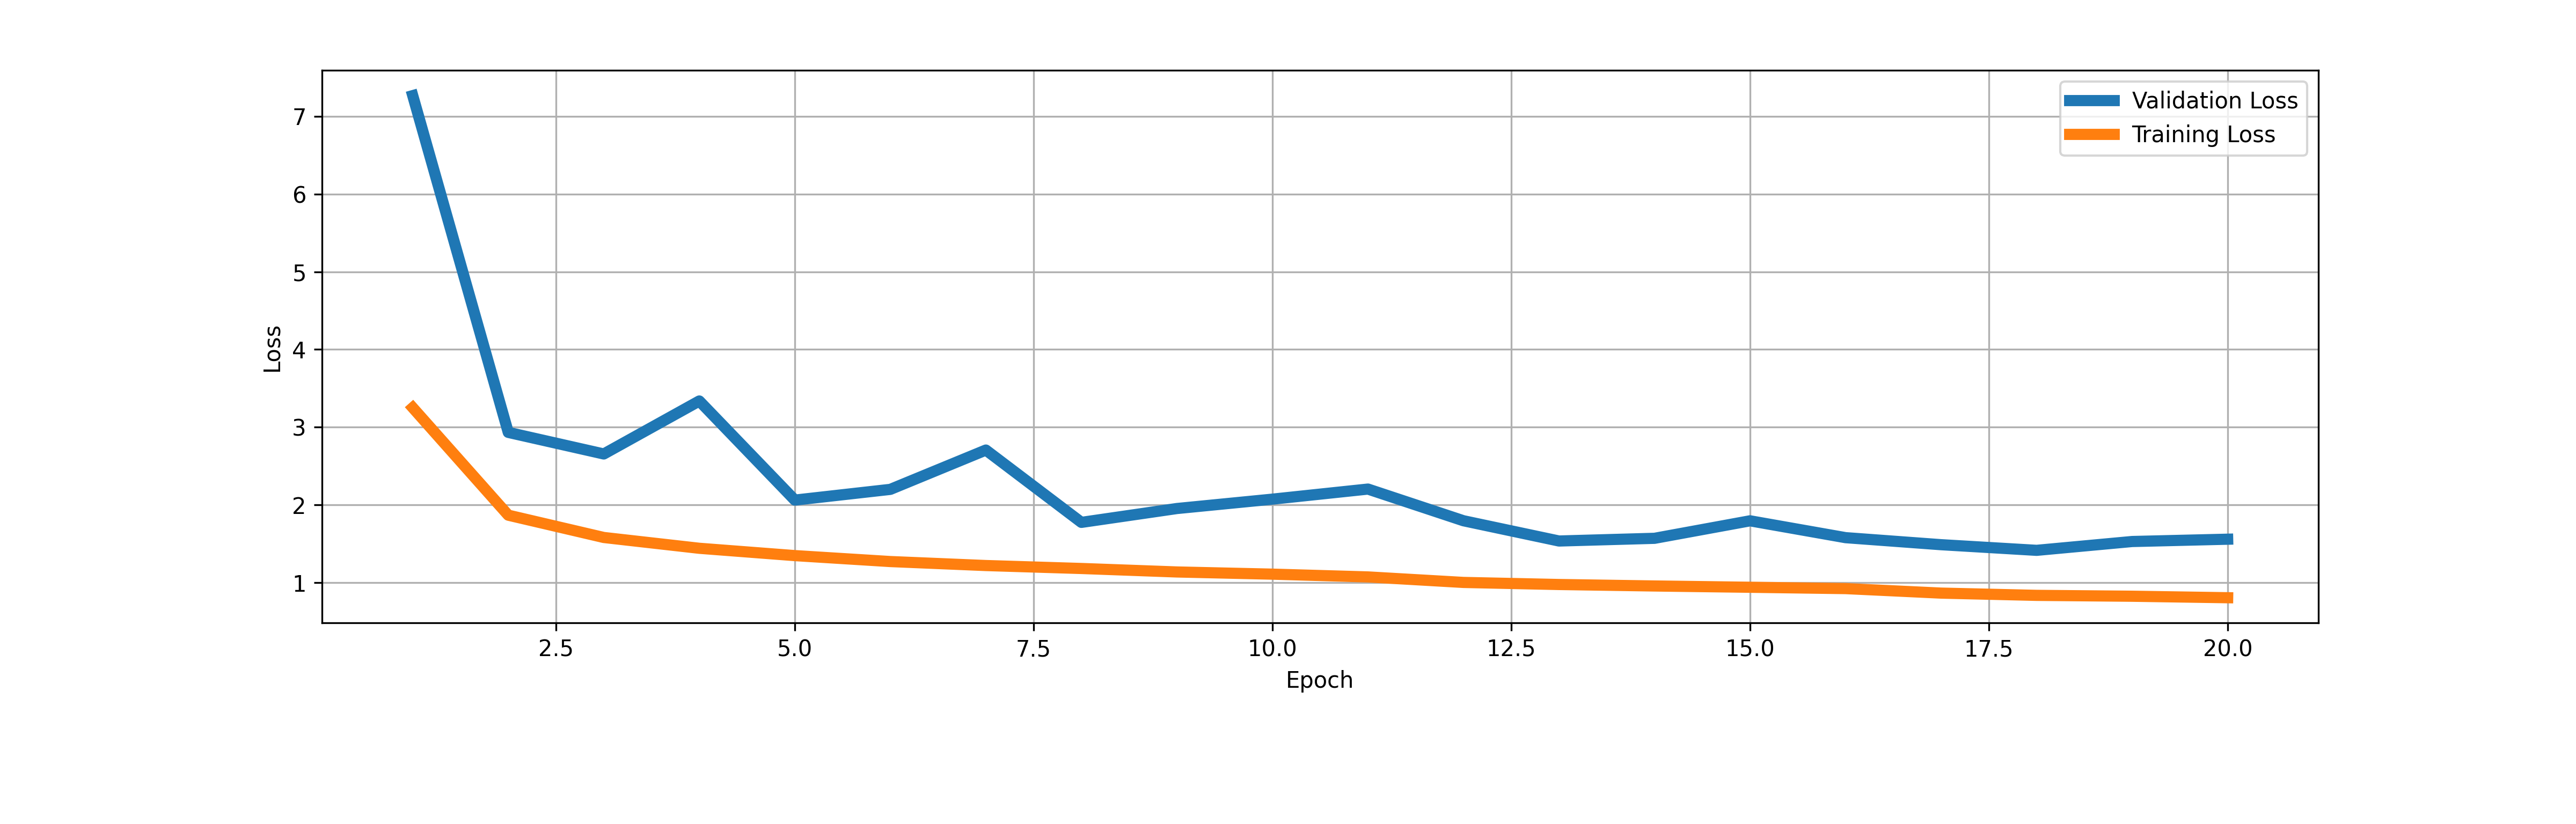
\includegraphics[width=0.95\linewidth]{680-loss.png}
    \caption{The Loss with batch size 680}
\end{figure}
\item Size of Training dataset \\
We have tried two kinds of sizes of training dataset with batch size 680, 
which are 1500 and 20000 data each category. We shuffled them into 340 files.
To prevent overfitting and overwhelming RAM, we train 10 epochs on the first one and 37 epochs on the second one.
On the one with smaller dataset, we can train over all data in one epoch.
However, in the one with larger dataset, 
we can only sample a part of them due to the validation set might be too large for RAM. 
The loss of the first one is around 1.5, and it overfits.
The loss of the second one is around 0.5, and it is not overfitting.
\begin{figure}[!htb]
    \centering
    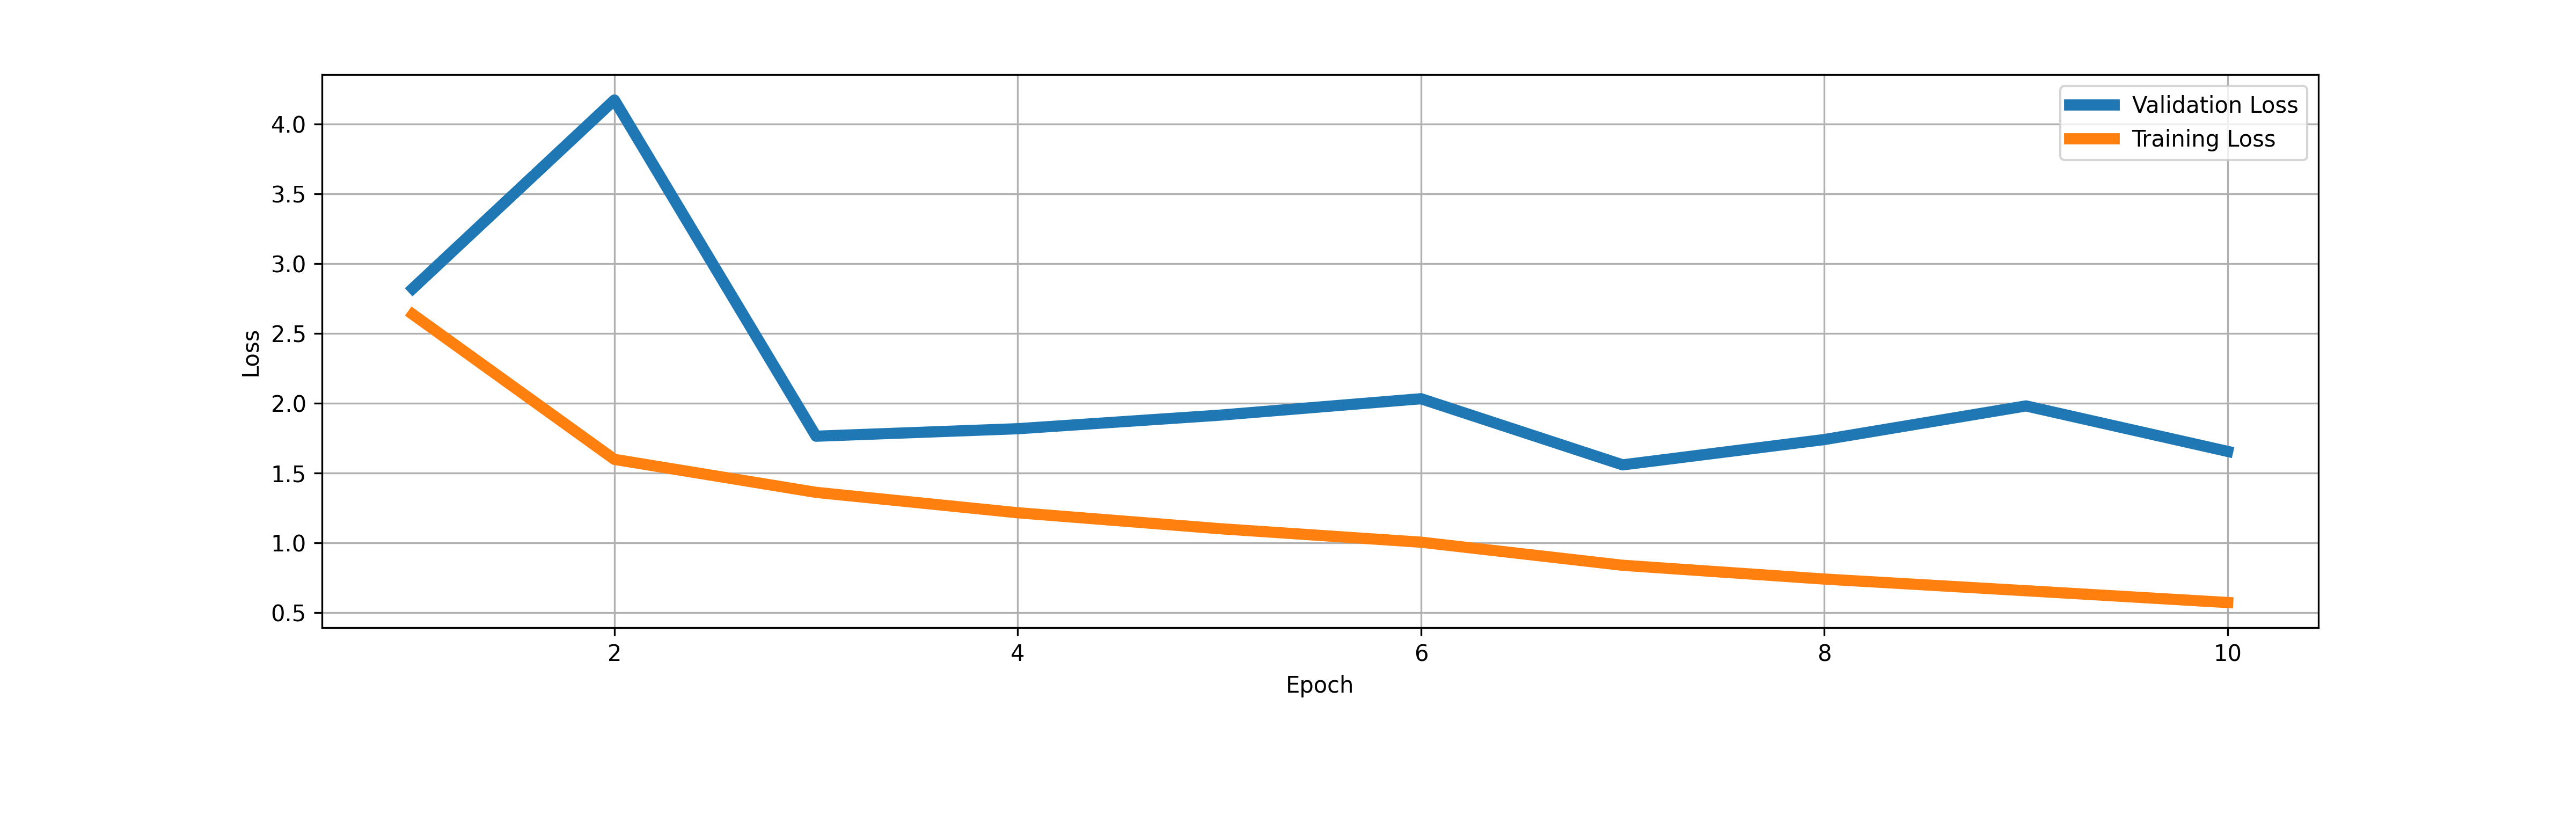
\includegraphics[width=0.95\linewidth]{1500-10.png}
    \caption{The Loss with 1500 data each category}
\end{figure}
\begin{figure}[!htb]
    \centering
    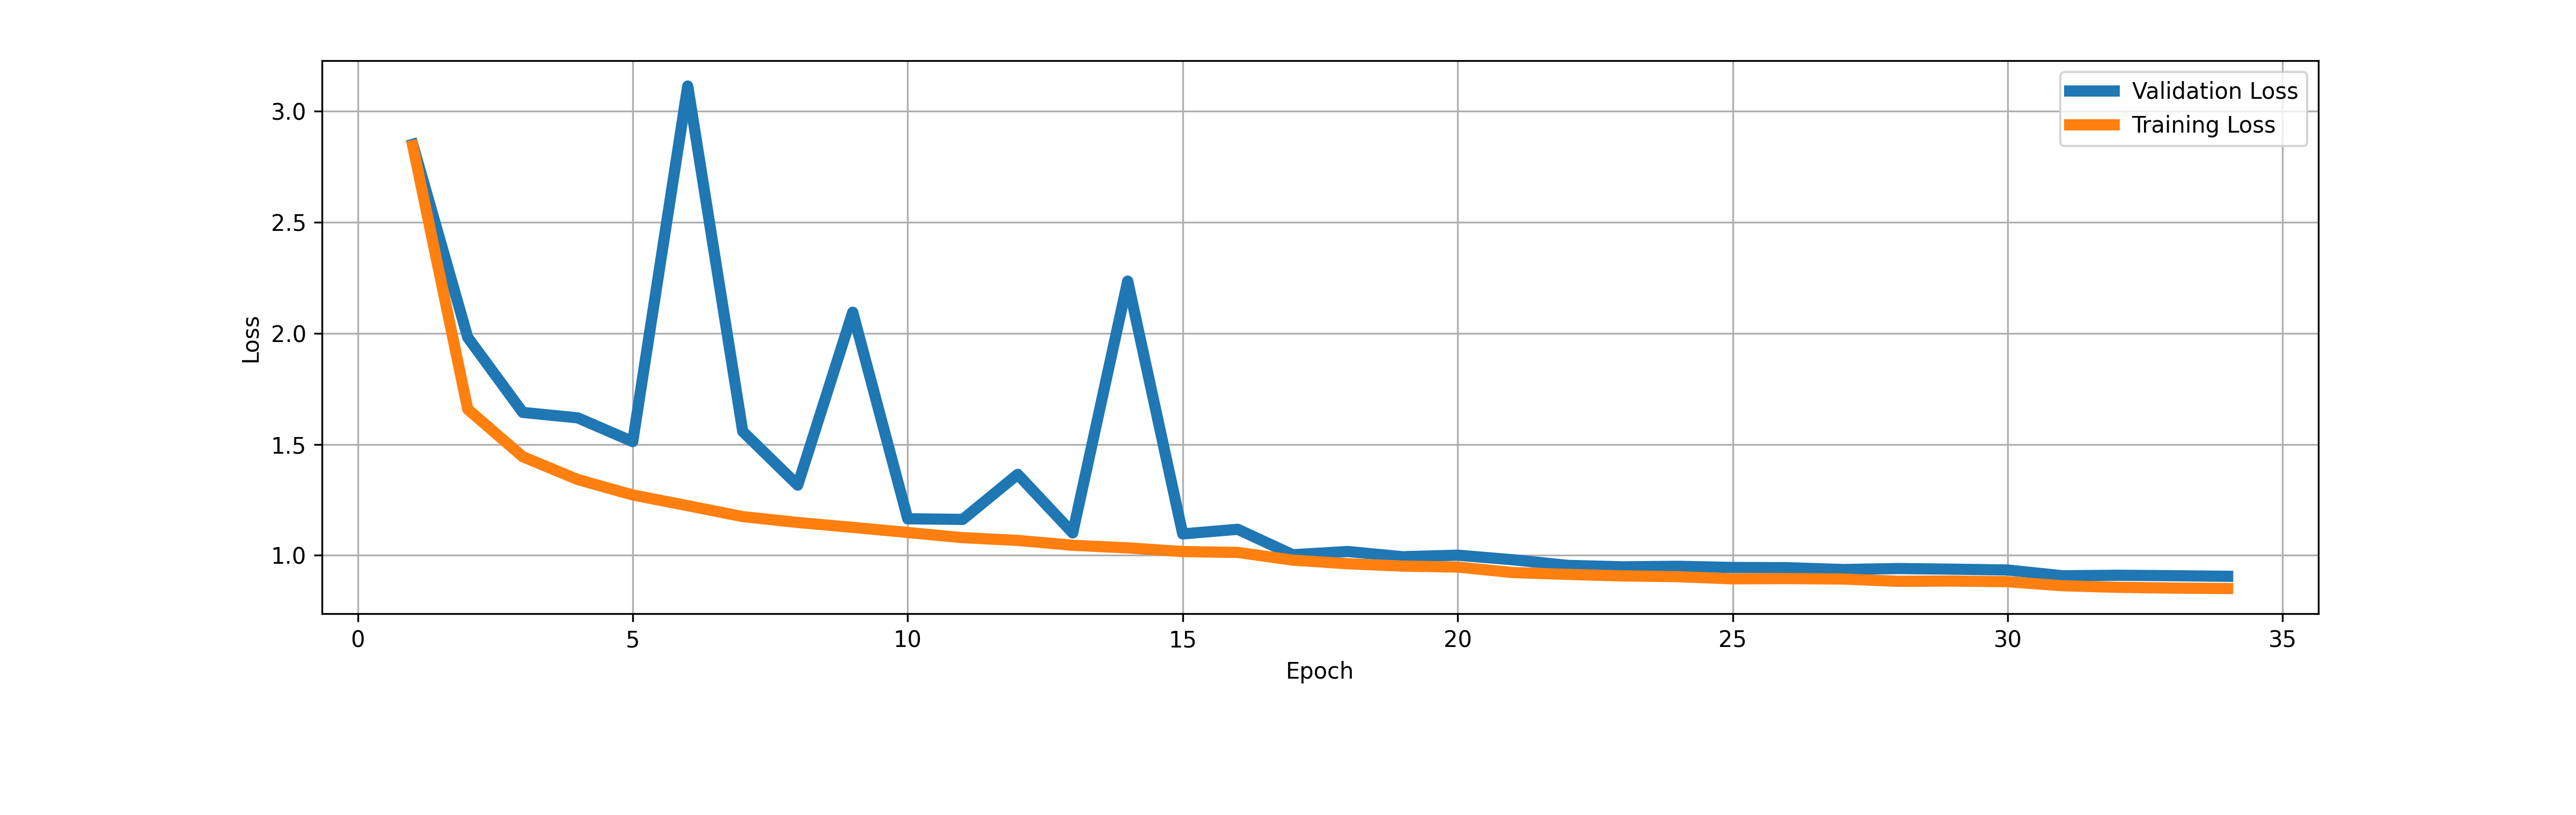
\includegraphics[width=0.95\linewidth]{20000-37.png}
    \caption{The Loss with 20000 data each category}
\end{figure}
\item Results \\
After comparing the results of different batch size and size of training dataset,
we found that the best way to train the model is to use a smaller batch size and a larger training dataset.
However, the time to train the model will be longer, so we need to find a balance between the time and the accuracy.
Because of the limited computing resources, we can not test for the whole dataset and neither can we train more epochs in a single session.
The best score we have got is 0.86151, which uses a batch size 340 and trains in over 30 epochs. Since the loss of validation set is still decreasing,
we can get higher scores if we increase the number of epochs in a single session.

\end{itemize}
\section{Other Information}
\begin{itemize}
\item Github Repo: \text{https://github.com/Mao-Siang/AI\_Final}
\item Video Link:
\item Contribution: \\
MaoSiang: 50\%, coding, data preprocessing, report. \\
ChengHsun: 50\%, coding, data preprocessing, video. \\
==
\end{itemize}
%-------------------------------------------------------------------------

%%%%%%%%% REFERENCES
{\small
\bibliographystyle{ieee_fullname} 
\bibliography{egbib}
% \bibliographystyle{IEEEtran,}
}

\end{document}
